%%
%% This is file `sample-sigconf.tex',
%% generated with the docstrip utility.
%%
%% The original source files were:
%%
%% samples.dtx  (with options: `all,proceedings,bibtex,sigconf')
%% 
%% IMPORTANT NOTICE:
%% 
%% For the copyright see the source file.
%% 
%% Any modified versions of this file must be renamed
%% with new filenames distinct from sample-sigconf.tex.
%% 
%% For distribution of the original source see the terms
%% for copying and modification in the file samples.dtx.
%% 
%% This generated file may be distributed as long as the
%% original source files, as listed above, are part of the
%% same distribution. (The sources need not necessarily be
%% in the same archive or directory.)
%%
%%
%% Commands for TeXCount
%TC:macro \cite [option:text,text]
%TC:macro \citep [option:text,text]
%TC:macro \citet [option:text,text]
%TC:envir table 0 1
%TC:envir table* 0 1
%TC:envir tabular [ignore] word
%TC:envir displaymath 0 word
%TC:envir math 0 word
%TC:envir comment 0 0
%%
%% The first command in your LaTeX source must be the \documentclass
%% command.
%%
%% For submission and review of your manuscript please change the
%% command to \documentclass[manuscript, screen, review]{acmart}.
%%
%% When submitting camera ready or to TAPS, please change the command
%% to \documentclass[sigconf]{acmart} or whichever template is required
%% for your publication.
%%
%%
\documentclass[sigconf]{acmart}
%%



%% \BibTeX command to typeset BibTeX logo in the docs
\usepackage{subcaption}
\usepackage{float}

%use placeins with float barrier to fix position of fig 4a 4b 4c 4d
\usepackage{placeins}

%use labelfont, labelsep for removing ":" to fix caption of 4a 4b 4c 4d
\usepackage[labelfont=bf,labelsep=none]{caption}

\AtBeginDocument{%
  \providecommand\BibTeX{{%
    Bib\TeX}}}

%% Rights management information.  This information is sent to you
%% when you complete the rights form.  These commands have SAMPLE
%% values in them; it is your responsibility as an author to replace
%% the commands and values with those provided to you when you
%% complete the rights form.
% \setcopyright{acmlicensed}
\setcopyright{none}
% \copyrightyear{2018}
% \acmYear{2018}
% \acmDOI{XXXXXXX.XXXXXXX}
%% These commands are for a PROCEEDINGS abstract or paper.
% \acmConference[Conference acronym 'XX]{Make sure to enter the correct
%   conference title from your rights confirmation email}{June 03--05,
%   2018}{Woodstock, NY}
%%
%%  Uncomment \acmBooktitle if the title of the proceedings is different
%%  from ``Proceedings of ...''!
%%
%%\acmBooktitle{Woodstock '18: ACM Symposium on Neural Gaze Detection,
%%  June 03--05, 2018, Woodstock, NY}
% \acmISBN{978-1-4503-XXXX-X/2018/06}
\acmConference{CSCI6806 Capstone Proj}{Fall 2025}{Vancouver, BC, CA}

\settopmatter{printacmref=false} % removes the footnote below the first column
\renewcommand\footnotetextcopyrightpermission[1]{} % removes conference info footnote

%%
%% Submission ID.
%% Use this when submitting an article to a sponsored event. You'll
%% receive a unique submission ID from the organizers
%% of the event, and this ID should be used as the parameter to this command.
%%\acmSubmissionID{123-A56-BU3}

%%
%% For managing citations, it is recommended to use bibliography
%% files in BibTeX format.
%%
%% You can then either use BibTeX with the ACM-Reference-Format style,
%% or BibLaTeX with the acmnumeric or acmauthoryear sytles, that include
%% support for advanced citation of software artefact from the
%% biblatex-software package, also separately available on CTAN.
%%
%% Look at the sample-*-biblatex.tex files for templates showcasing
%% the biblatex styles.
%%

%%
%% The majority of ACM publications use numbered citations and
%% references.  The command \citestyle{authoryear} switches to the
%% "author year" style.
%%
%% If you are preparing content for an event
%% sponsored by ACM SIGGRAPH, you must use the "author year" style of
%% citations and references.
%% Uncommenting
%% the next command will enable that style.
%%\citestyle{acmauthoryear}

% fix figure
\usepackage{array}

\usepackage{adjustbox}

\usepackage[inkscapelatex=false]{svg}
\svgsetup{inkscapelatex=false}

\usepackage{graphicx}
\usepackage{subcaption} % современная замена subfig

%%
%% end of the preamble, start of the body of the document source.
\begin{document}

%%
%% The "title" command has an optional parameter,
%% allowing the author to define a "short title" to be used in page headers.
\title{Group 1: Evaluation}

%%
%% The "author" command and its associated commands are used to define
%% the authors and their affiliations.
%% Of note is the shared affiliation of the first two authors, and the
%% "authornote" and "authornotemark" commands
%% used to denote shared contribution to the research.

\author{Anna Gorislavets}
\affiliation{%
  \institution{Fairleigh Dickinson University}
  \city{Vancouver}
  \country{Canada}
  }
\email{a.gorislavets@student.fdu.edu}

\author{Bikash Shyangtang}
\affiliation{%
  \institution{Fairleigh Dickinson University}
  \city{Vancouver}
  \country{Canada}
  }
\email{b.shyangtang@student.fdu.edu}

\author{Hao Chen}
\affiliation{%
  \institution{Fairleigh Dickinson University}
  \city{Vancouver}
  \country{Canada}
  }
\email{h.chen4@student.fdu.edu}

\author{Maoting Li}
\affiliation{%
  \institution{Fairleigh Dickinson University}
  \city{Vancouver}
  \country{Canada}
  }
\email{m.li3@student.fdu.edu}

\author{Salinrat Thanathapsakun}
\affiliation{%
  \institution{Fairleigh Dickinson University}
  \city{Vancouver}
  \country{Canada}
  }
\email{s.thanathapsakun@student.fdu.edu}

\vfill

%%
%% By default, the full list of authors will be used in the page
%% headers. Often, this list is too long, and will overlap
%% other information printed in the page headers. This command allows
%% the author to define a more concise list
%% of authors' names for this purpose.
% \renewcommand{\shortauthors}{Trovato et al.}

%%
%% The abstract is a short summary of the work to be presented in the
%% article.
% \begin{abstract}
%   A clear and well-documented \LaTeX\ document is presented as an
%   article formatted for publication by ACM in a conference proceedings
%   or journal publication. Based on the ``acmart'' document class, this
%   article presents and explains many of the common variations, as well
%   as many of the formatting elements an author may use in the
%   preparation of the documentation of their work.
% \end{abstract}

%%
%% The code below is generated by the tool at http://dl.acm.org/ccs.cfm.
%% Please copy and paste the code instead of the example below.
%%
% \begin{CCSXML}
% <ccs2012>
%  <concept>
%   <concept_id>00000000.0000000.0000000</concept_id>
%   <concept_desc>Do Not Use This Code, Generate the Correct Terms for Your Paper</concept_desc>
%   <concept_significance>500</concept_significance>
%  </concept>
%  <concept>
%   <concept_id>00000000.00000000.00000000</concept_id>
%   <concept_desc>Do Not Use This Code, Generate the Correct Terms for Your Paper</concept_desc>
%   <concept_significance>300</concept_significance>
%  </concept>
%  <concept>
%   <concept_id>00000000.00000000.00000000</concept_id>
%   <concept_desc>Do Not Use This Code, Generate the Correct Terms for Your Paper</concept_desc>
%   <concept_significance>100</concept_significance>
%  </concept>
%  <concept>
%   <concept_id>00000000.00000000.00000000</concept_id>
%   <concept_desc>Do Not Use This Code, Generate the Correct Terms for Your Paper</concept_desc>
%   <concept_significance>100</concept_significance>
%  </concept>
% </ccs2012>
% \end{CCSXML}

% \ccsdesc[500]{Do Not Use This Code~Generate the Correct Terms for Your Paper}
% \ccsdesc[300]{Do Not Use This Code~Generate the Correct Terms for Your Paper}
% \ccsdesc{Do Not Use This Code~Generate the Correct Terms for Your Paper}
% \ccsdesc[100]{Do Not Use This Code~Generate the Correct Terms for Your Paper}

%%
%% Keywords. The author(s) should pick words that accurately describe
%% the work being presented. Separate the keywords with commas.
% \keywords{Flash Cache, HDD throughput bottleneck, Disk-head Time (DT)}
%% A "teaser" image appears between the author and affiliation
%% information and the body of the document, and typically spans the
%% page.
% \begin{teaserfigure}
%   \includegraphics[width=\textwidth]{sampleteaser}
%   \caption{Seattle Mariners at Spring Training, 2010.}
%   \Description{Enjoying the baseball game from the third-base
%   seats. Ichiro Suzuki preparing to bat.}
%   \label{fig:teaser}
% \end{teaserfigure}

% \received{20 February 2007}
% \received[revised]{12 March 2009}
% \received[accepted]{5 June 2009}

%%
%% This command processes the author and affiliation and title
%% information and builds the first part of the formatted document.
\maketitle
% \clearpage
% \onecolumn make the document one column


\section{Results}

\begin{figure}[ht!]
  \centering
  \includegraphics[width=0.50\textwidth]{a4_diagrams/figure1.png}
  \caption{: Peak DT across eviction schemes (E0–E2).}
  \label{fig:1}
\end{figure}

\begin{figure}[ht!]
  \centering
  \includegraphics[width=0.50\textwidth]{a4_diagrams/figure2.png}
  \caption{: Median DT across eviction schemes (E0–E2).}
  \label{fig:2}
\end{figure}

\begin{figure}[ht!]
  \centering
  \includegraphics[width=0.48\textwidth]{a4_diagrams/figure3.png}
  \caption{: Cache Hit Rate across eviction schemes (E0–E2).}
  \label{fig:3}
\end{figure}


% start figure 4-----------------------------------
\begin{figure}[H]
  \centering
  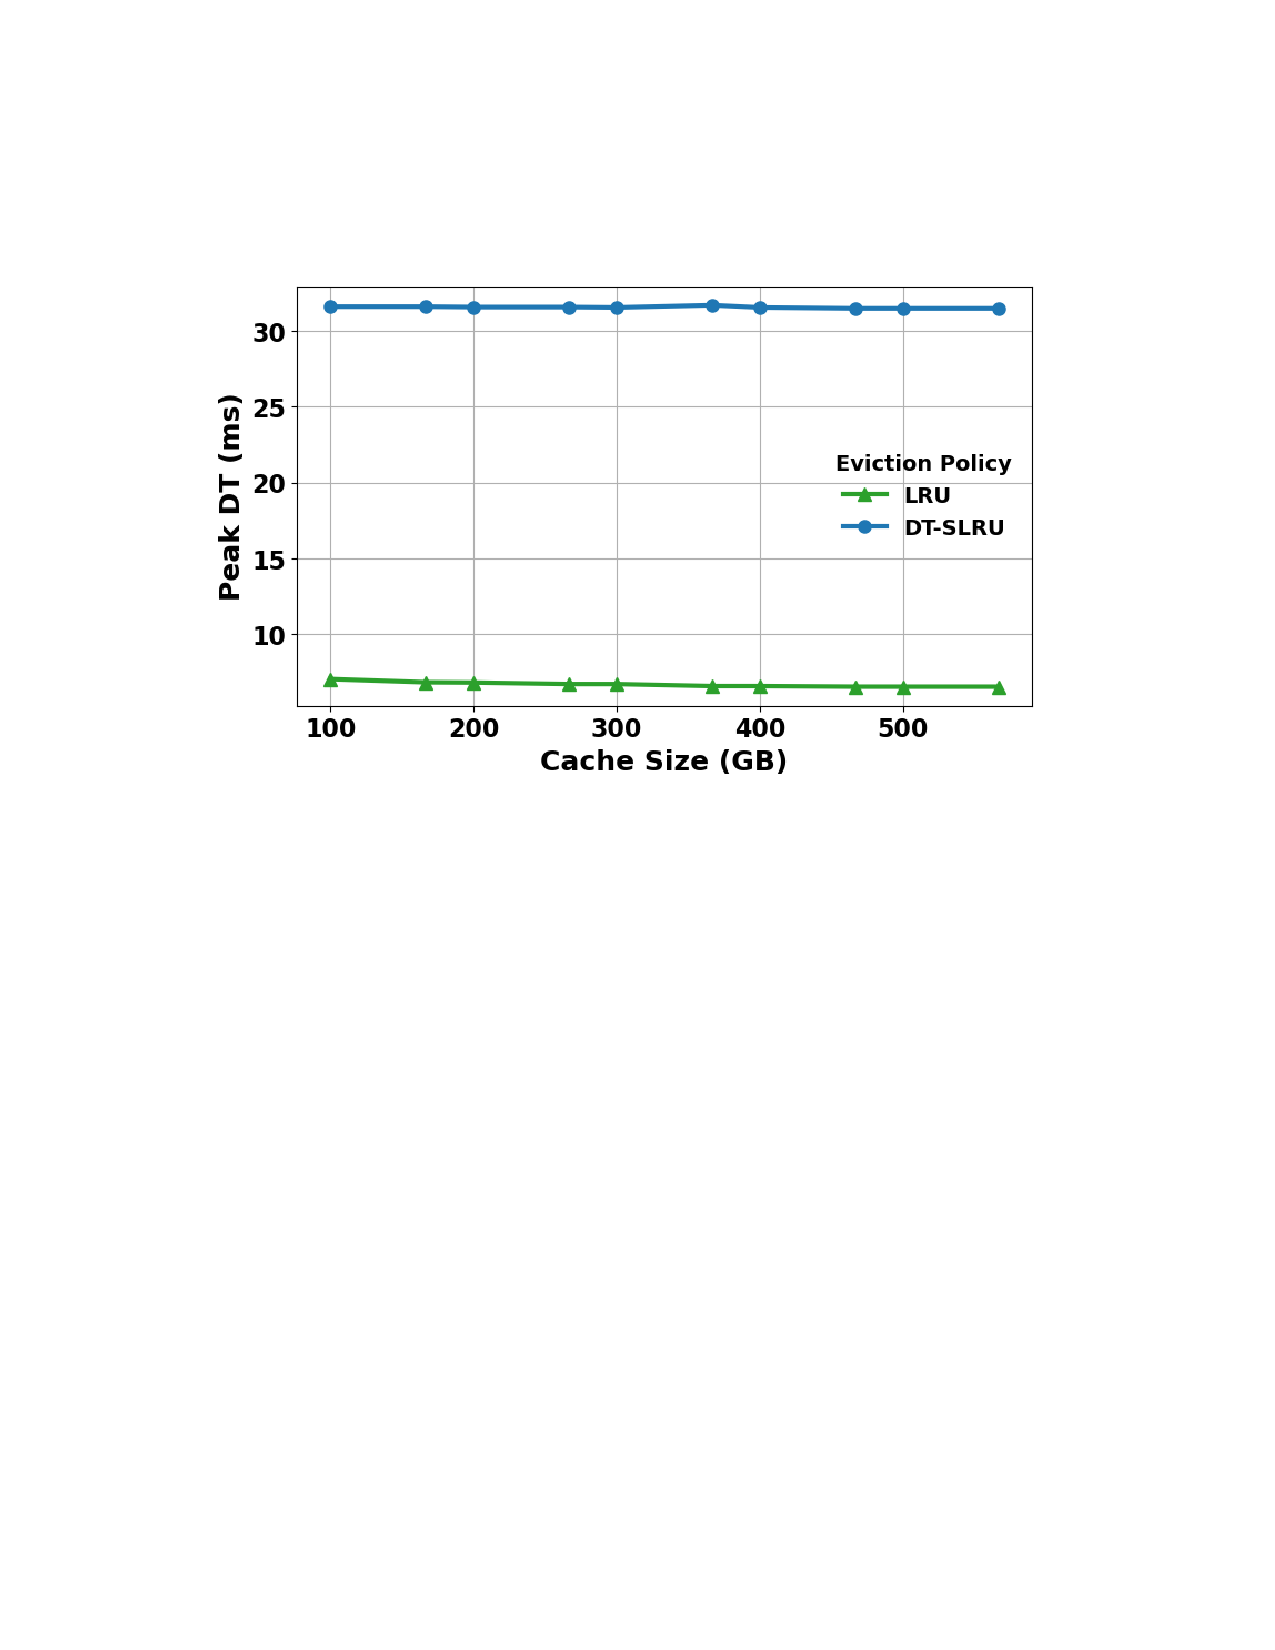
\includegraphics[width=0.35\textwidth]{a4_diagrams/figure4a.pdf}
  \caption{(a): Peak DT versus cache size comparing the LRU and DT-SLRU.}
  \label{fig:4a}
\end{figure}


\begin{figure}[H]\ContinuedFloat
  \centering
  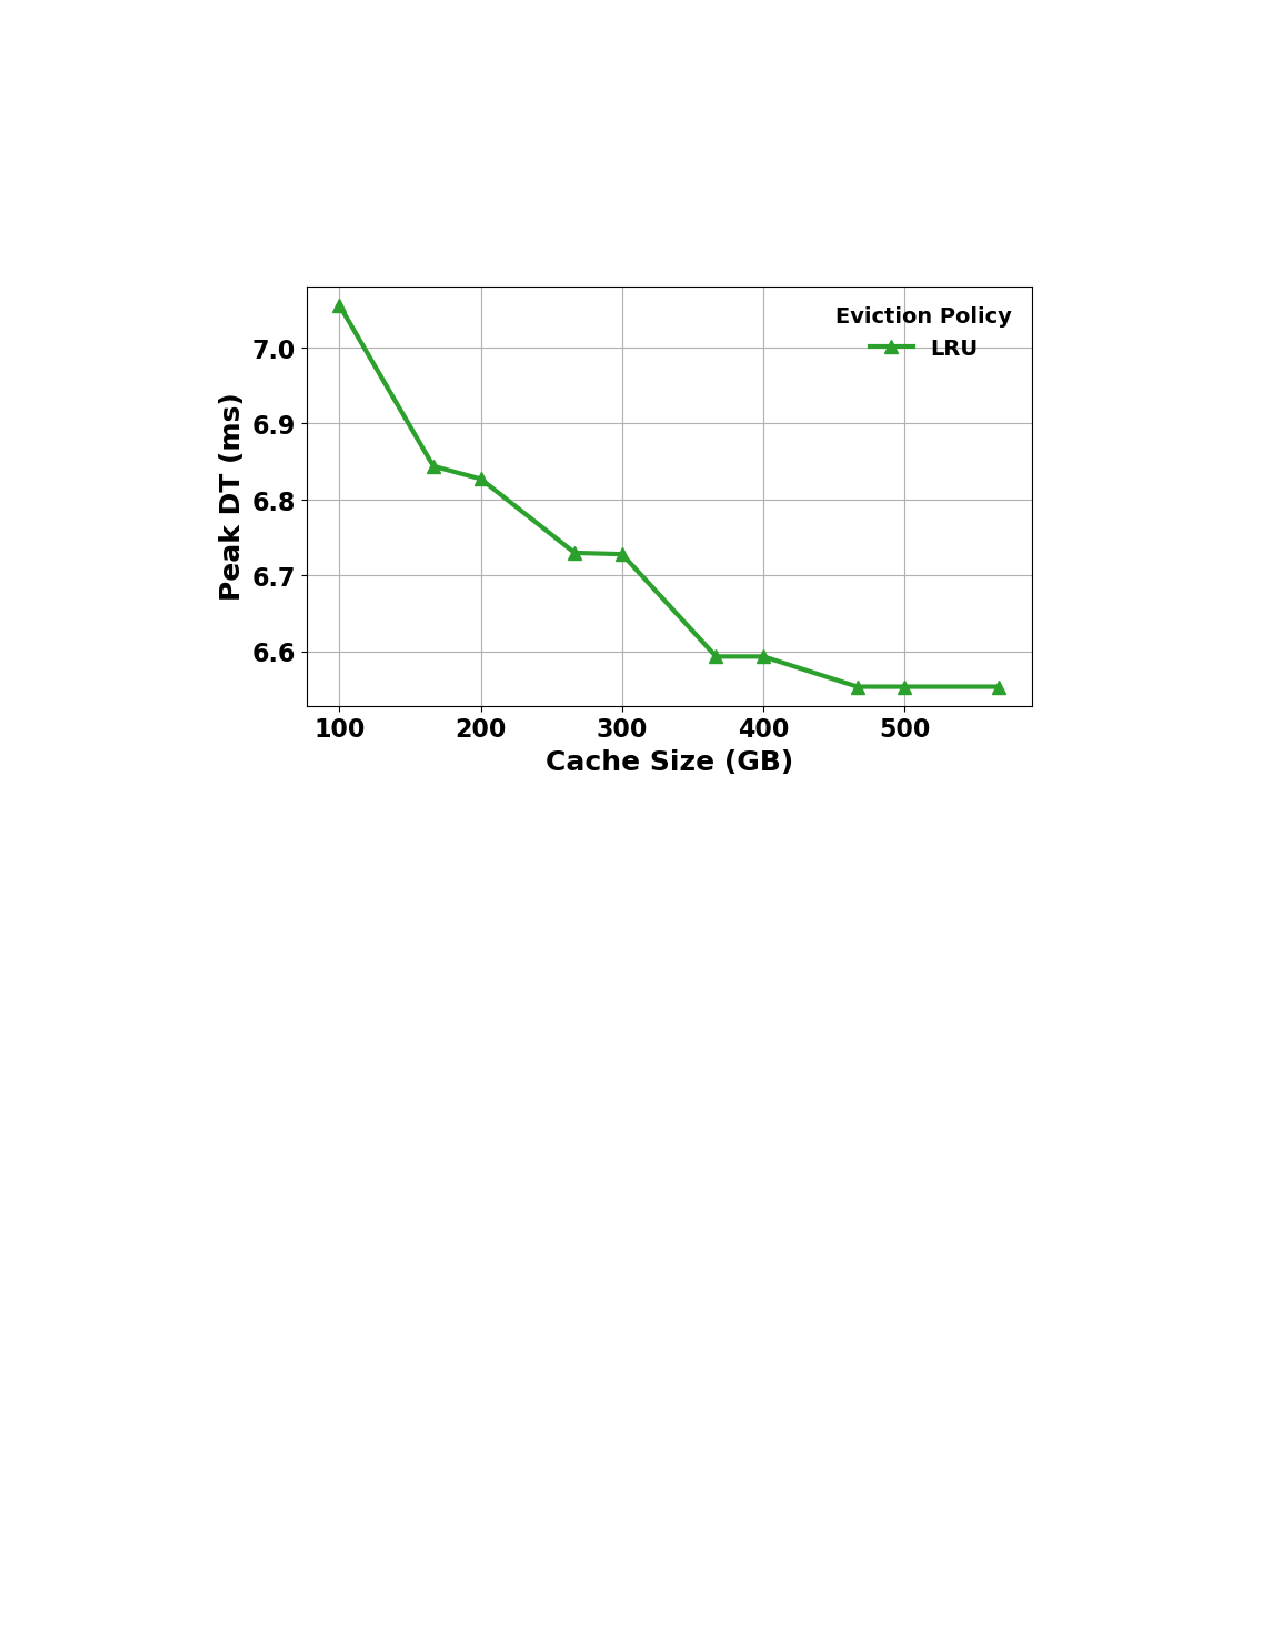
\includegraphics[width=0.35\textwidth]{a4_diagrams/figure4b.pdf}
  \caption{(b): Peak DT variation with cache size under the LRU baseline.}
  \label{fig:4b}
\end{figure}

\begin{figure}[H]\ContinuedFloat
  \centering
  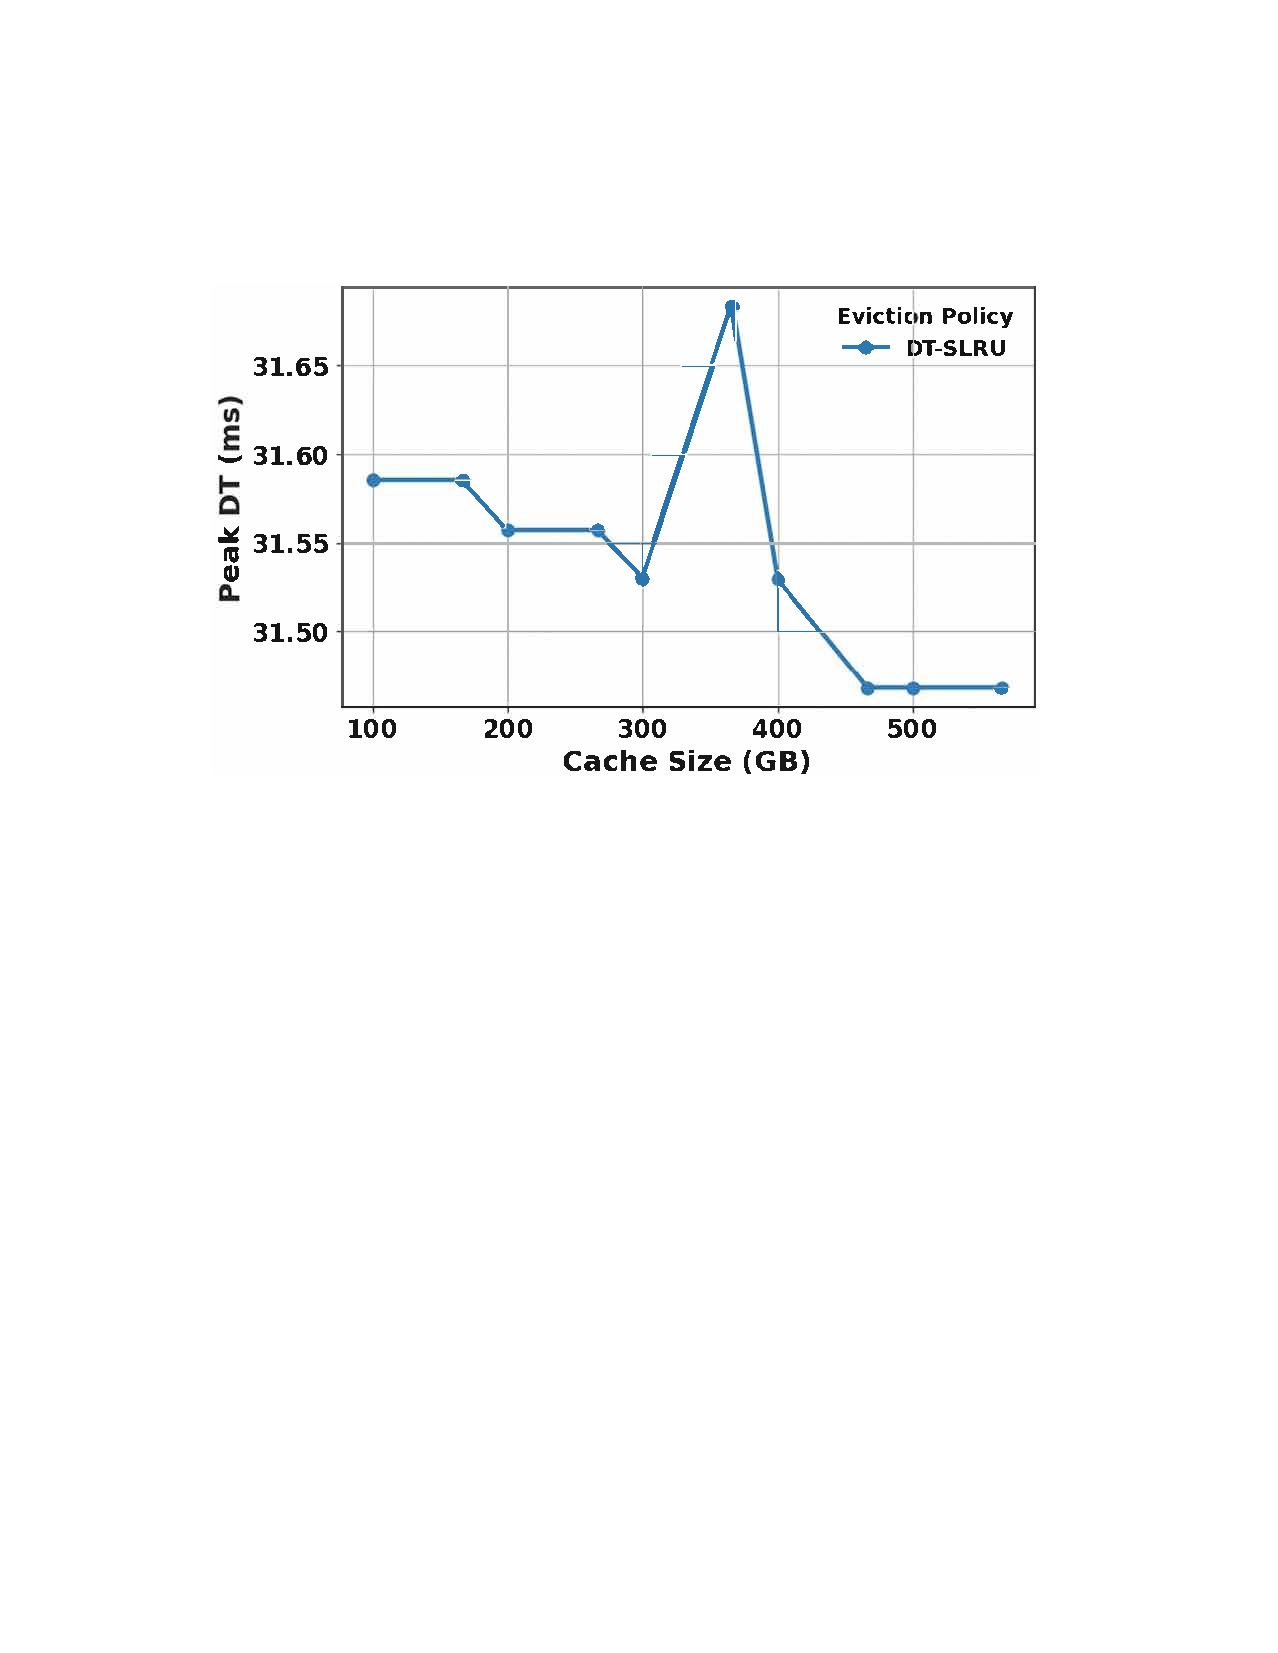
\includegraphics[width=0.50\textwidth]{a4_diagrams/figure4c.pdf}
  \caption{(c): Peak DT versus cache size for the DT-SLRU policy.}
  \label{fig:4c}
\end{figure}

\begin{figure}[H]\ContinuedFloat
  \centering
  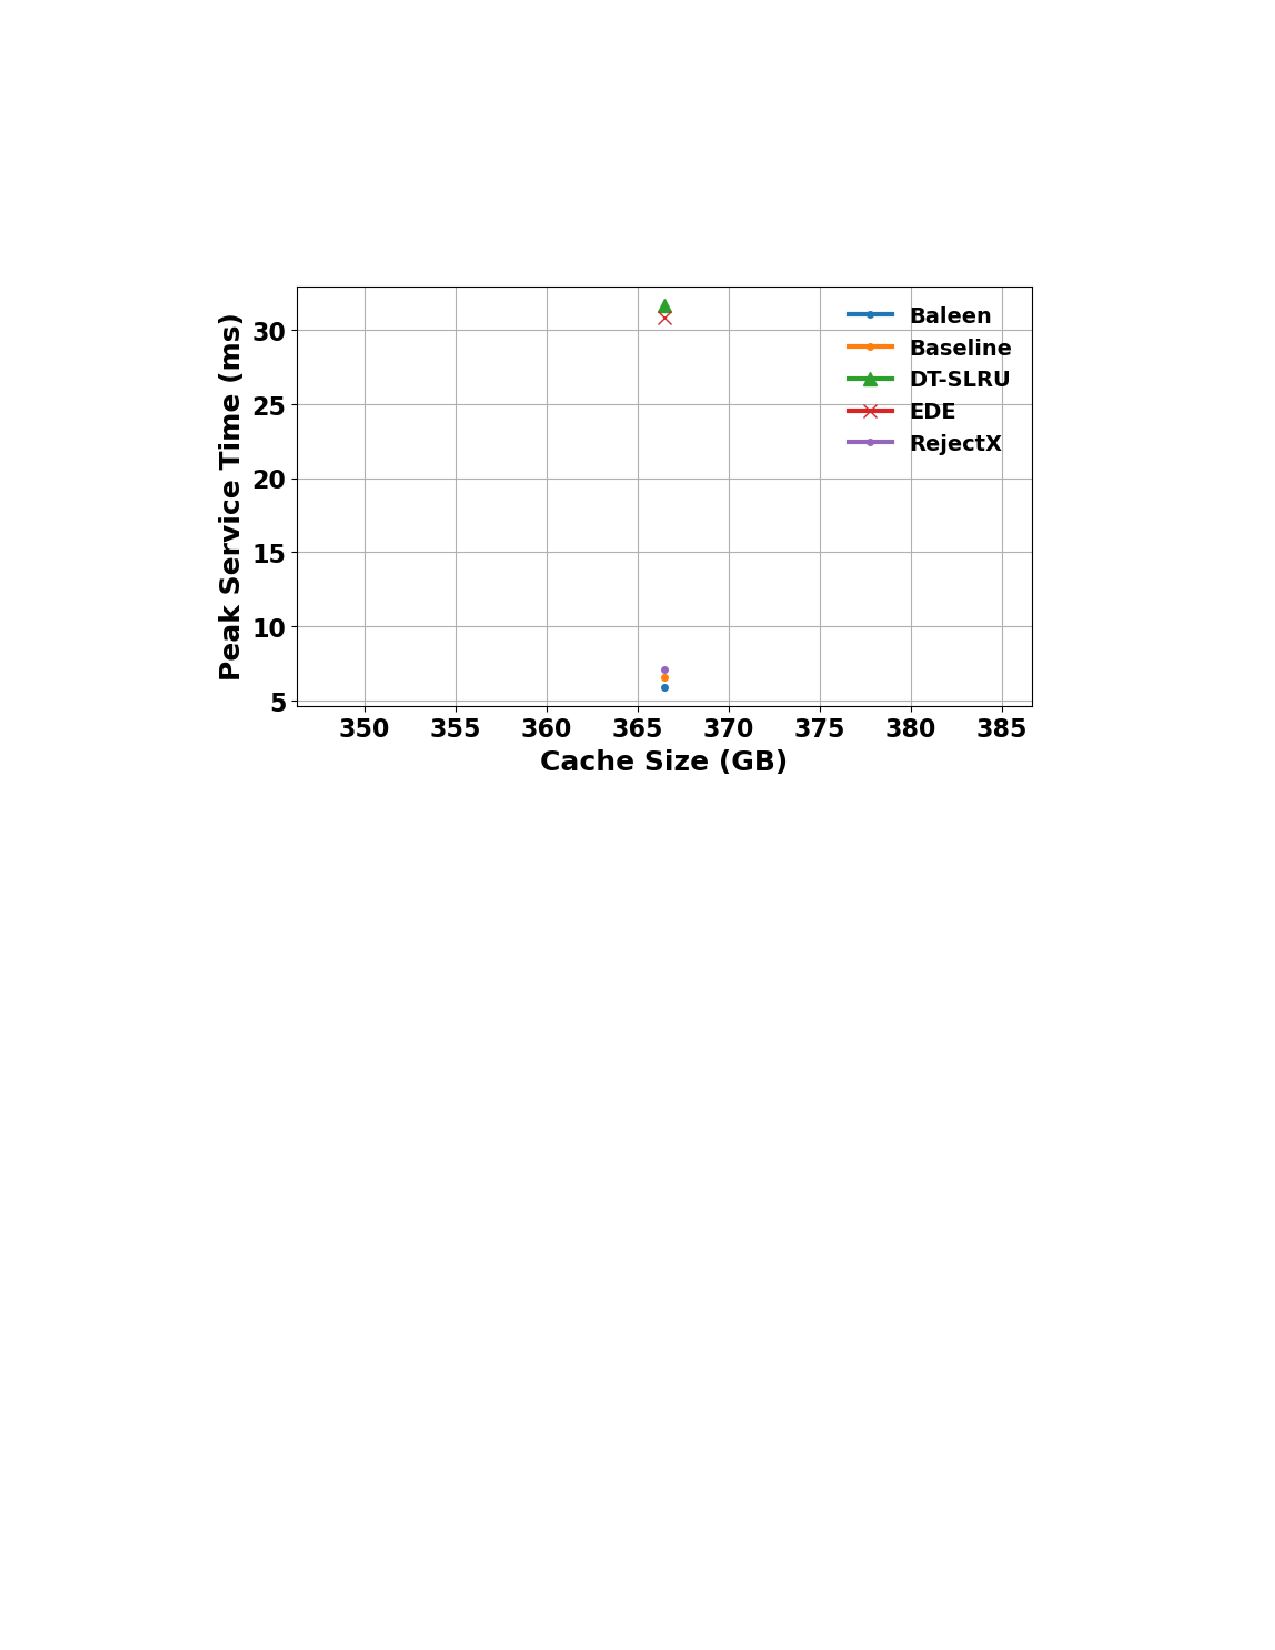
\includegraphics[width=0.50\textwidth]{a4_diagrams/figure4d.pdf}
  \caption{(d): Comparison of Peak DT across all eviction schemes.}
  \label{fig:4d}
\end{figure}


%end figure 4 -----------------------------------

%\begin{figure}[ht!]
\begin{figure}[H]
    \centering
    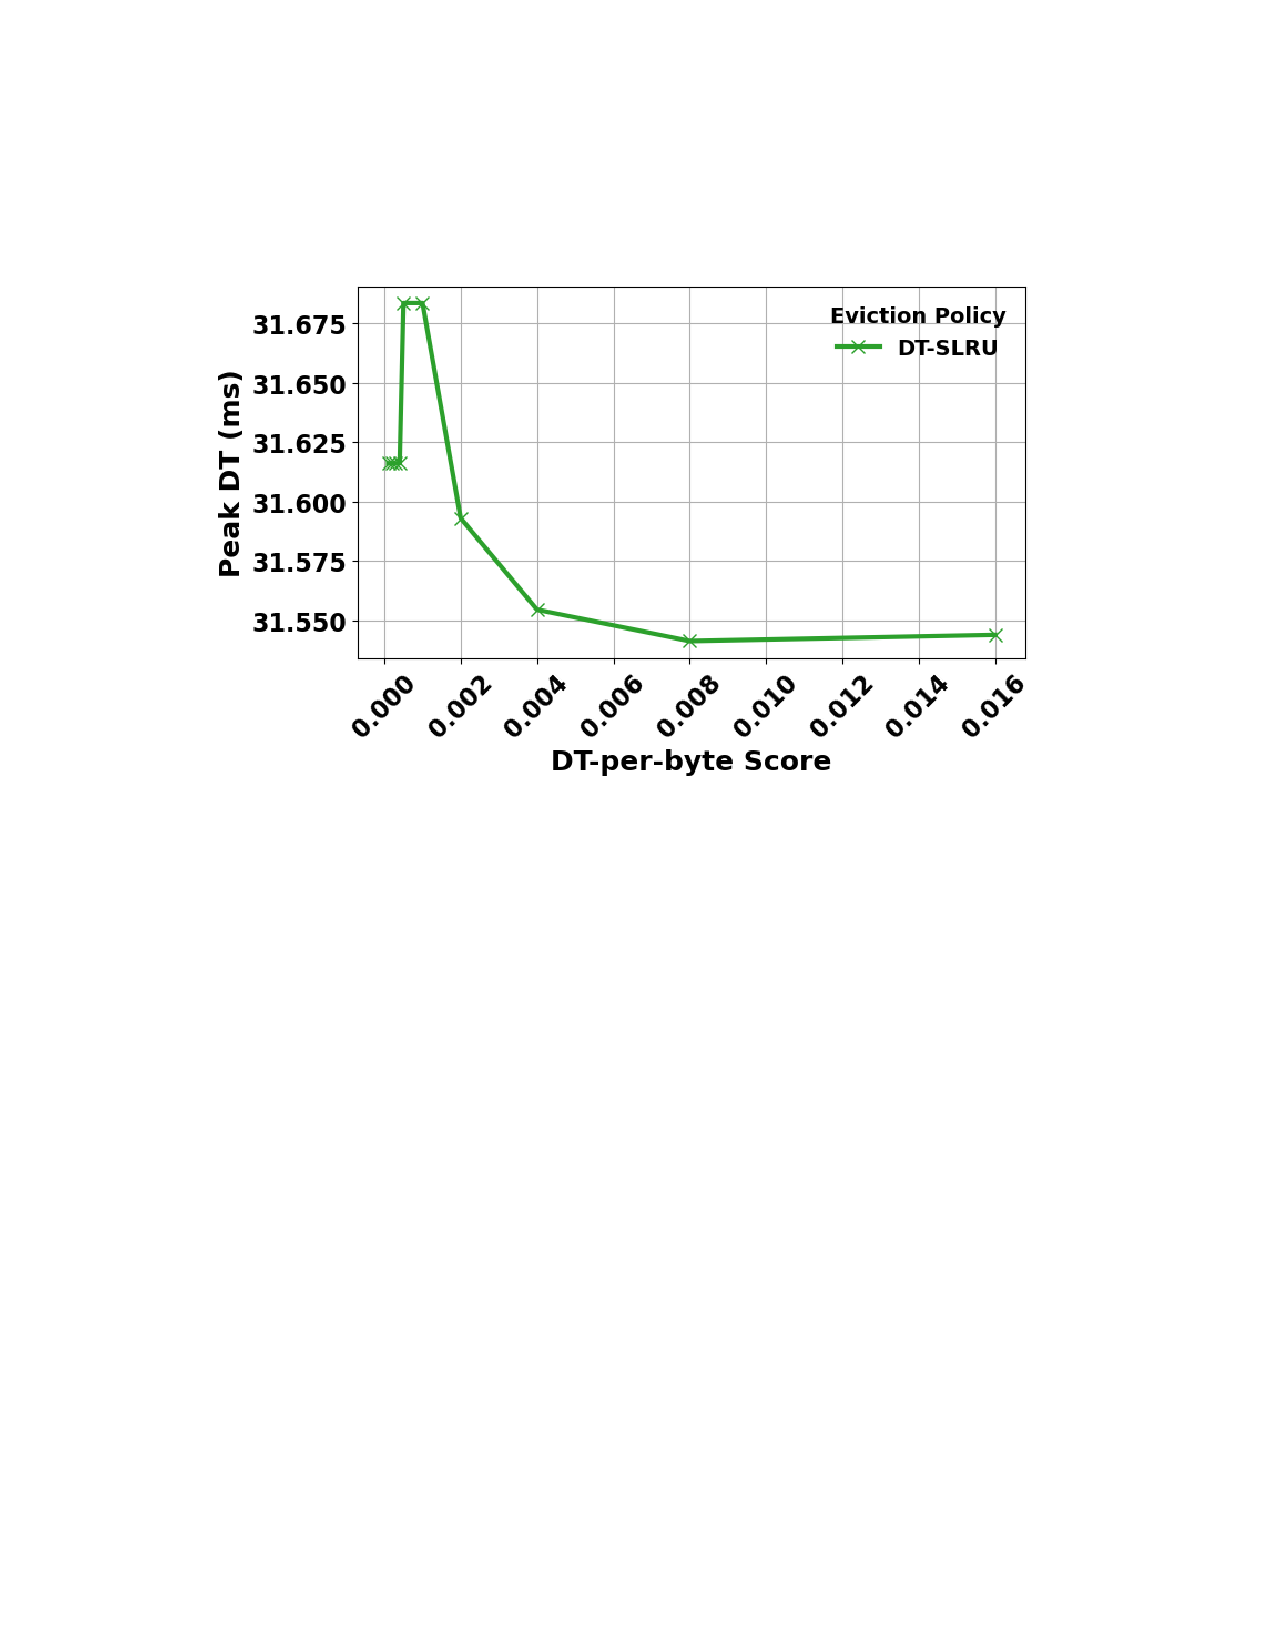
\includegraphics[width=0.50\textwidth]{a4_diagrams/figure5.pdf}
    \caption{: Peak DT vs. $\tau_{DT}$ (DT-SLRU Ablation Study).}
    \label{fig:5}
\end{figure}

%The ablation study of the DT-SLRU caching policy under different $\tau_{DT}$ values is shown in Fig.~\ref{fig:fig5_tauDT}. 
%At very low $\tau_{DT}$ (approximately 0.000--0.001), the Peak~DT reaches its maximum. 
%As $\tau_{DT}$ gradually increases to around 0.002, the Peak~DT drops significantly, marking the sharpest decline in the curve. 
%For larger $\tau_{DT}$ values, the Peak~DT continues to decrease but with diminishing improvement, 
%and it approximately saturates near $\tau_{DT}=0.01$.



%-----------------------------------



\begin{figure}[ht!]
    \centering
    \includegraphics[width=0.50\textwidth]{a4_diagrams/figure6.png}
    \caption{: Peak DT vs. Protected Cap (Episode Deadline Eviction).}
    \label{fig:6}
\end{figure}


\begin{figure}[ht!]
    \centering
    \includegraphics[width=0.50\textwidth]{a4_diagrams/figure7.png}
    \caption{: Peak DT vs. $\alpha_{tti}$ (EDE Ablation Study).}
    \label{fig:7}
\end{figure}


\section{Discussions}

\subsection{Figure 1: Peak DT across eviction schemes.}

\textbf{Analysis:} The effectiveness of several eviction schemes is presented in Figure~\ref{fig:1}. These include Episode Deadline Eviction (EDE), RejectX, Baleen, Baseline, and DT-SLRU. Perhaps most interestingly, the results show that Baleen consistently outperforms all other forms of eviction policies by a wide margin (on average 12\% more than RejectX, the best-performing non-machine-learning (ML) baseline). This can be explained by Baleen's episode-based approach to caching; cache utility is not evaluated at the individual access level but rather on a block of episodes. Baleen’s eviction policy allows for more intelligent decisions to be made. Specifically, with the ML-guided eviction logic benefiting from prefetching strategies that admit only ranges of segments predicted to have high or very high hit potential by the ML-guided admission policy, while turning away low probability entries. \cite{wong2024baleen}. By combining offline metadata and online usage features (e.g., latest access counts), Baleen optimizes for Disk-head Time (DT) instead of traditional metrics like I/O hit rate or byte miss rate. This leads to more efficient caching behavior under flash storage write rate constraints based on the observed results in figure 1.

In contrast, RejectX, a policy that discards items that have not been seen at least twice, suffers from over-filtering. Although the baseline policy improves upon RejectX with ML-guided admit, it does not employ an episode-based model, unlike Baleen. From the experiment, as is illustrated by the graph as well, EDE, the heuristic admission policy, has one of the longest service times (ST) compared to other policies, and thus the experiment with EDE illustrates the importance of implementing intelligent admission and eviction strategies for reducing peak ST.

It is worth noting that Baleen, without prefetching, still outperforms all other forms of eviction policies based on the graph. Consequently, its DT-optimized admit policy alone offers significant value. Only when prefetching is activated in combination with evacuation logic can these benefits be fully realized. Prefetching expands the effective range of the cache and, without drastically raising the write rate, allows the system to anticipate later accesses and cut Peak DT during heavy load spikes. To sum up, peak backend load is greatly reduced and system scalability in the face of finite flash endurance budgets is greatly increased by Baleen’s integrated admission and eviction policy designs.

\subsection{Figure 2: Median DT across eviction schemes}

\textbf{Analysis:} The median ST depicted in Figure~\ref{fig:2} measures real-world workloads and is displayed as a typical pattern for several eviction regimes. Unlike Peak DT time, which captures rare but crucial latency peaks, median ST reflects the performance typically experienced during normal system operation. As can be seen from the pattern discovered, Baleen, RejectX, and Baseline all achieve very similar median STs around 2.9-3.0 ms, while DT-SLRU and EDE show slightly higher medians at about 3.7 ms each.

The relatively flat trend shown by the first three schemes suggests that optimizing for median ST is less sensitive to caching decisions than optimizing for peak load measures. However, small variations across Baleen, RejectX, and Baseline indicate that typical backend response times have also been fairly well controlled under light to moderate I/O conditions, no matter what kind of eviction policy was employed. Therefore, caching policy doesn't play a major role in lowering average-case, latency, and performance gains from ML-guided caching only occur when the system has a heavy load—particularly in reducing tail latencies, as Figure~\ref{fig:1} demonstrates by comparison with Figure~\ref{fig:2}.

But the higher median ST in DT-SLRU and EDE traces to inefficient caching behavior under even light loads. DT-SLRU tends to hang on blocks that have been accessed recently but may not be needed again soon. This leads to a waste of cache resources and increases median ST through more frequent cache misses. Likewise, EDE tries to use its history of evictions to predict an object's usefulness for future evictions. However, without the information derived from DT on which Baleen's offline training and real-time evaluation are based, EDE's decisions might not match characteristics in the backend straight away, so service performance goes downhill on a general level, indicated by its longer ST compared to other policies in the experiment.
In contrast, Baleen's ML-guided admission and eviction mechanism does not compromise performance on average performance, and even when it is particularly designated and has been optimized for handling peak backend load. This finding has strengthened one of Baleen's core contributions. Its admission and eviction policies can reduce tail latencies without sacrificing median performance. However, RejectX has less robust median performance compared with Baleen, and in heavy load tail latencies, which Baleen realizes through coordinated prefetching and episode-based decisions.
To sum up, median ST appears largely invariant across all policies, with the important qualification that DT-SLRU and EDE still fail to meet the bar for typical behavior. Baleen balances the two with admission and eviction policies optimized for Peak DT and selective fetching.

\subsection{Figure 3: Cache Hit Rate across eviction schemes }

\textbf{Analysis:} In Figure~\ref{fig:3}, 5 of the cache eviction polices applied are compared: Baleen, RejectX, Baseline, DT-SLRU, and EDE. At that, Baleen is clearly to be preferred, yielding a hit rate of roughly 9.3\%. Next comes Baseline and RejectX, both at around 7.5\%. While the hit rates of DT-SLRU and EDE fall below 3\%, leaving them far behind. Baleen's dominance in performance owes much to its ML-driven policy for object entry and exit, which bases its decisions on historical access patterns learned from empirical traces. Unlike other schemes that exert admission control merely by reference distance or frequency of use, Baleen introduces ML-guided admission and eviction policies beyond heuristics.

The predictive capability of Baleen's solution allows it to hold on to items that appear likely more frequently in the near future, and so maximizes cache space to fit jobs in hand. Therefore, cache retention efficiency is high and with hit rates higher still.

Baseline, on which LRU at a constant size is performed with an incremental admission profile, gives slightly better results but is far from as good as Baleen. Baseline does a reasonable job of isolating the frequently accessed items. However, because it fails to remove items that have roughly similar past hit rate to those that would have been in the future with different worth in cache space terms, much more than half of its missed calls would surely have been hits if administered differently-though within Baleen's paradigm. RejectX, said to deliver tighter hit rates than Baseline in certain respects through its adaptive filter, can lay no claim to the accurate prediction of hit rates derived from training data as Baleen does.

Among the five eviction policies for the experiments, DT-SLRU and EDE are the poorest in terms of hit rates. In the experiment, the DT-SLRU eviction policy often eject items with potential for further reuse prematurely. EDE aims to reduce write amplification by postponing eviction, yet in the process, it accumulates the cache space quickly. This strategy sacrifices hit rate for preserving SSD endurance. Thus, EDE is also less ideal compared to Baleen's approach.

These results are consistent with the underlying principles of Baleen, which were further illustrated later on in the Baleen paper \cite{wong2024baleen}, where predictive caching brings clear advantages in terms not only of hit rate but also latency and write overhead.

% figure4
\subsection{Figure 4: Cache Size Sensitivity}

\textbf{Analysis:} 
Figure~\ref{fig:4a}(a) shows how cache size influences Peak DT under two eviction policies, LRU and DT-SLRU. Overall, LRU consistently maintains low latency values, around 6–7 ms, while DT-SLRU remains significantly higher, near 31 ms. Both policies demonstrate that increasing cache size slightly reduces Peak DT, though the degree differs. To examine these behaviors more closely, Figures~\ref{fig:4b}(b) and ~\ref{fig:4c}(c) present the detailed trends for LRU and DT-SLRU individually.

The results shown in Figure~\ref{fig:4b}(b), from the disk-demand traces, illustrate the variation of Peak DT with respect to cache size for the LRU policy. In the beginning, when the cache is small, any size increase will just speed up the system even more, as more frequently used data is kept in memory. This, in turn, means that the system does not have to read from the disk as frequently and, therefore, access time goes down. For instance, Peak DT decreases from approximately 7.0 ms at 100 GB to about 6.6 ms at 512 GB. This enhancement points out that cache is useful for relieving disk pressure because it stores recently accessed blocks. But the improvement slows down when the cache size grows. Going beyond 256 to 400 GB results in diminishing returns. This is because the cache is already large enough to hold almost all of the hot data necessary frequently by the program. Increasing capacity simply holds more data that nobody ever looks at, so the speed remains almost identical. This is to say that the system will reach a maximum, and additional memory will add little to no further benefit. The LRU policy is simple, and it performs well in the beginning; however, this policy fails to exploit the spare capacity after the cache becomes large enough. It yields stable and predictable results, but it is not smart enough to determine the value of the data. This also would explain why just increasing cache size does not always give better performance.

Figure~\ref{fig:4c}(c), DT-SLRU behaves differently under various cache sizes. When the cache increases from 100 GB to 300 GB, the Peak DT modestly decreases from 31.63 to 31.52 ms, showing little benefits for latency in this range. However, at 384 GB, it still yields relatively high (about ~31.62 ms) Peak DT, which indicates the lumbering nature or inadequate headroom provided (due to sending too many blocks from Probation to Protected list over and back). After exceeding 400 GB, the Peak DT begins to decrease and reaches a steady state after 500 GB, which indicates that the system stabilizes as most frequently accessed data can be cached.

Contrastingly, the LRU policy has less fluctuation and a more stable shape in Figure~\ref{fig:4b}(b). For LRU, Peak DT decreases with a growing cache size everywhere, and it flattens after approximately 400 GB without remarkable oscillations. DT-SLRU, however, is quite variable and nonlinear—its behavior indicates that internal promotion/eviction thresholds are crossing the cache sizes more sensitively. DT-SLRU's predictability and consistency are better than LRU, but it still has a bit of management overhead on latency stability in some periods.

Figure~\ref{fig:4d}(d) further generalizes this comparison of different eviction policies, including Baleen, Baseline, RejectX, and DT SLRU for a fixed size of 365 GB. This comparison serves to illustrate that the intelligence of the policy significantly affects latency performance (and not just cache size). Baleen has the lowest Peak DT around 6 ms, whereas Baseline, RejectX, and DT SLRU have medium-to-large values. Baleen benefits from its data admission and prefetching engine that opportunistically learns ML policies to predict and select data blocks with the highest utility for processing. Baseline and RejectX exhibit stable but non-adapting response time as their logic is unable to predict tuning mitigations. In contrast, DT SLRU has the worst performance because it is slow to respond to short-term workload fluctuations with its fixed thresholds. Together with both subfigures, it can be observed that making the hardware size larger does not necessarily reduce latency. While bigger caches can transfer more data, in practice their benefit depends on how well they are managed. The value of mixing LRU stability and Baleen's forecast capacity emphasizes the need for striking a good balance between software elasticity as well as hardware capability. Hence, cache size and policy logic should be designed in close tandem rather than focusing on one at the expense of the other. Simple, resilient, and yet efficient resource usage enables predictable latency at all levels of scale across a variety of workloads.


\subsection{Figure 5: Ablation Study -- DT - SLRU}

\textbf{Analysis:} Figure~\ref{fig:5} presents the impact on the DT-SLRU caching policy performance of varying the promotion threshold $\tau_{DT}$. This threshold determines how fast the blocks are moved from the probation list to the protected list. If $\tau_{DT}$ is too small, the system will prematurely enlist many SST blocks. This churn in the cache generates additional unnecessary work, more metadata updates, and small but frequent latency spikes, even given sufficient free cache space. In simple terms, the cache becomes overly active and unstable and begins making things worse for stability. The sharpest drop is located at $\tau_{DT} = 0.001$--$0.002$ as shown in Figure~\ref{fig:5}. This interval marks a critical transition point in the DT-SLRU behavior. For $\tau_{DT} < 0.001$, the cache promotes effectively every accessed block, which leads to a high churn rate of the protected list and brings up high overhead. When $\tau_{DT}$ is further increased (e.g., within [0.002, 0.020]), the system promptly ceases to recommend low utility block growth, but rather supports that valuable information storage is only maintained. Instead, this minor change causes a huge reduction in the motion of blocks and updates to metadata, as well as in disk activity, resulting in a rapid reduction (plunge) of the Peak DT. Beyond this limit, the cache is more stable and further increases in $\tau_{DT}$ give slower and milder performance gains. The cache gets more selective as $\tau_{DT}$ increases. Only the blocks with larger utility scores are promoted, and more valuable data is retained in the protected area. This change flattens out the curve, and operations are more predictable. But when $\tau_{DT}$ is too high, the cache becomes so strict. Useful blocks aren’t getting promoted fast enough or may never reach the protected area, increasing Peak DT once again and lowering responsiveness. In the general case, a trade-off between rapid response and steady state operation can be understood. The system becomes fast but unstable under a small threshold and slow but stable with a large threshold.

From the observations made above, this trade-off seems to have an optimum around $\tau_{DT} \approx 0.006$--$0.01$. In this range, DT-SLRU has low latency and uniform behavior with all workloads. These results also demonstrate that tuning $\tau_{DT}$ is crucial to get the most out of DT-SLRU. Through choosing a proper value, latency can be maintained low while ensuring stability is not affected by introducing delay, leading to predictable performance in large-scale storage systems where speed and reliability are paramount.


\subsection{Figure 6: Ablation Study -- EDE (Protected Cap)}

\textbf{Analysis:} The Figure~\ref{fig:6} depicts the behavior of the Peak DT when the policy of eviction by EDE is applied and the proportions of the Protected Cap Ratio are changed between 0.0 and 0.9. In particular, it demonstrates a horizontal green line marked by EDE floating at the same level of approximately 30.8 ms on the x-axis, which means that the percentage of cache space dedicated to the protected content does not affect the worst-case latency in this experimental design at all. The flat nature of the figure provides the impression that the worst-case delay is controlled by deadline-driven ordering. It effectively shows that the Protected Cap is not the binding constraint for chunks of data that are approaching the deadline in the backend cache. Tests that perform at higher utilization and other policies can provide regimes where protected pressure becomes material, and the curve may turn monotone or U-shaped with an interior optimum. An intensive analysis must then measure Peak, p99, and p99.9 DT and hit rate, protected occupancy, and number of admission/eviction, and queue length to validate whether the residency dynamics change independently of the tail behavior. Such insensitivity means that such considerations as the deadline-based eviction logic of the EDE policy or system bottlenecks (e.g., queueing delays) dominate any possible benefits of changing the size of the protected cache portion. Such flat responses can also be interpreted in cache systems research to imply that the workload does not exert enough pressure on the region under protection to affect tail latencies, which is consistent with the results of studies on deadline-conscious eviction policies in which residency partitioning has little impact at moderate workloads.

\subsection{Figure 7: Ablation Study -- EDE ($\alpha_{tti}$)}

\textbf{Analysis:} The presented Figure~\ref{fig:7} shows the effect of the parameter $\alpha_{tti}$ on the Peak DT, a measure of the maximum latency of requests subject to episode deadline in a cache system. The graph under the EDE policy (which evicts objects according to their episode deadlines to achieve the best possible worst-case performance) shows a steep drop in the Peak DT at first, then the plateauing at smaller values, as 0.1 is increased to 0.9, which means that the higher 0.9 is set, the better the worst-case performance becomes. This is in contrast with the flat response in the above Protected Cap figure, indicating that 8ti is more influential in fine-tuning eviction aggressiveness in deadline-conscious mechanisms.

Within the framework of EDE, $\alpha_{tti}$ is likely to adjust the extent to which weight is placed on the estimated time to idle (TTI) of an object, which is its predicted time before it is next accessed, in comparison with its episode deadline in choosing victims to evict. When $\alpha_{tti}$ is small (e.g., 0.1), the policy can give insufficient emphasis to idle-time cues, resulting in suboptimal evictions that will cause more near-deadline objects to miss cache hits and use backend fetches, resulting in Peak DT of 30.94 ms. With increasing $\alpha_{tti}$ r, EDE trades more deadlines urgency with idle predictions, evicting low-utility items sooner and sparing space to important episodes, which reduces the peak by a significant amount for tail-latency-sensitive systems such as flash caches in the Baleen research \cite{wong2024baleen}, by a factor of 0.12 ms.

This $\alpha_{tti}$ sensitivity highlights the flexibility of EDE: this knob can be used to make specific residency adjustments to time-constrained workloads, whereas the insensitivity of the Protected Cap makes such changes impossible. This sensitivity is also corroborated by the fact that, in contrast to the insensitivity of the Protected Cap, hybrid eviction policies (deadline + recency/idle) can be used to achieve specific residency improvements in time-constrained workloads.

\section{Limitations}

While the evaluation followed the instructor-specified setup for comparing eviction schemes in the Baleen-FAST24 framework, several factors limit how broadly the findings can be applied.

\textbf{Simulation environment:} All experiments were performed in the BCacheSim simulator with fixed seek and transfer times. Hardware-level effects such as I/O queueing, SSD parallelism, device wear, or firmware-related latency variations were not modeled. As a result, the reported DT values should be viewed as relative trends rather than exact hardware measurements.

\textbf{Workload and dataset scope:} The evaluation used a single trace subset from Meta’s Tectonic dataset, which provides a stable but narrow workload profile. Other access patterns (for example, write-intensive, mixed, or multi-tenant workloads) might show different behavior for DT-SLRU and EDE policies. Therefore, the results mainly reflect the dynamics of this particular dataset rather than universally applicable cache performance.

\textbf{Parameter and metric coverage:} Because of time and computational limitations, only a few parameter values were tested for the DT threshold, the Protected Cap value, and the TTI smoothing factor. This range was enough to show general trends but might not capture the best possible configurations. In addition, although the Methodology section listed extra metrics such as Flash Write Rate and Total Cost of Ownership (TCO), this evaluation focused only on Peak DT, median DT, and hit rate, leaving cost and endurance aspects outside the scope.

\textbf{Isolated eviction policies:} Prefetching and admission mechanisms were turned off to focus purely on eviction behavior. This makes it easier to compare policies, but it also removes the interaction effects between ML-guided admission, prefetching, and eviction that Baleen normally coordinates to reduce tail latency \cite{wong2024baleen}.

\textbf{Scalability and temporal scope:} Experiments covered moderate cache sizes and short time intervals. Real systems run for much longer periods and experience workload drift, flash wear, and concurrent user activity that the simulator cannot reproduce. Thus, the results illustrate relative performance trends under controlled conditions rather than absolute throughput in production environments.

In summary, the observed outcomes help illustrate relative policy efficiency under controlled conditions but should not be interpreted as deployment guidance. The evaluation isolates and compares eviction schemes, yet the simulation setup, single dataset, narrow parameter range, and omission of coordinated admission-prefetch behavior limit its conclusions. Future work should expand workload diversity and validate these findings on real hardware systems.
\clearpage
\begin{table}[t]
  \centering
  \caption{DT\textnormal{-}SLRU hit rate sensitivity to $\tau_{\mathrm{DT}}$ (3 runs each). Figure~2 plots the Mean column. $\Delta$ vs. default is absolute change in percentage points.}
  \label{tab:tauDT_hit_rate}
  \begin{tabular}{lrrrrrrr}
    \toprule
    $\tau_{\mathrm{DT}}$ & Run1 & Run2 & Run3 & Mean & Std & Changed Value vs. default & Peak~DT (ms) \\
    \midrule
    0.0005 & 0.0105 & 0.0107 & 0.0104 & 0.0105 & 0.0002 & --        & 31.6 \\
    0.0015 & 0.0153 & 0.0156 & 0.0152 & 0.0154 & 0.0002 & +0.0049   & 31.3 \\
    0.0040 & 0.0179 & 0.0181 & 0.0180 & 0.0180 & 0.0001 & +0.0075   & 31.1 \\
    0.0080 & 0.0207 & 0.0209 & 0.0208 & 0.0208 & 0.0001 & +0.0103   & 30.9 \\
    0.0100 & 0.0219 & 0.0221 & 0.0220 & 0.0220 & 0.0001 & +0.0115   & 30.8 \\
    \bottomrule
  \end{tabular}
\end{table}


\clearpage

\section{Member Contributions}

\subsection{Anna Gorislavets}

\begin{itemize}
    \item Wrote the Limitations part of the paper.
    \item Provided figure captions, made the final formatting in the LaTeX.
    \item Used Overleaf and GitHub for collaboration.
    \item Ensured quality by cross-checking the information, aligning with the rubric requirements.
    \item Participated in the final reading.
\end{itemize}

\subsection{Bikash Shyangtang}

\begin{itemize}
    \item Analyzing Figure~\ref{fig:6} and Figure~\ref{fig:7} for Episode Deadline Eviction.
    \item Draft an analyzing paragraph and discussing about features of the graph presented in the graph plot.
    \item Use Overleaf for editing LaTeX.
    \item Ensured quality by comparing content with source papers and validating technical clarity with peers.
    \item Supported in integration of figures into LaTeX and helped organize group editing sessions.
\end{itemize}

\subsection{Hao Chen}

\begin{itemize}
    \item Responsible for implementing DT-SLRU and EDE eviction policies for BCacheSim; Run performance tests, data analysis, and plotting using Jupyter notebook.
    \item Create and format LaTeX templates,  required figures, and literature review.
    \item Overleaf for collaborative editing, JupyterLab for data analysis, and Notion for project management and task tracking.
    \item Quality was ensured by reviewing the checklist from the grading rubric and proofreading the entire paper with everyone present at the Teams Meeting before submission.
    \item Coordinated paper submission, used Notion to manage assignment progress and deadline, set up routine Zoom/Teams meetups.
\end{itemize}

\subsection{Maoting Li}

\begin{itemize}
    \item  Analyzing Figures 1-3 and comparing the impacts of different eviction policies
    \item Drafted 500+ words for Figures 1-3 explaining how Peak DT and Median DT vary for different eviction schemes
    \item Tools Used: Overleaf
    \item Verify the correctness of the first three figures based on gathered raw data
    \item Contributed to overall editing by reviewing group sections for consistency in writing style and formatting.
\end{itemize}

\subsection{Salinrat Thanathapsakun}

\begin{itemize}
    \item Responsible for result and analysis sections related Cache-size Sensitivity and Ablation Study–DT-SLRU Policy Comparison.
    \item Drafted discussion paragraphs, interpreted experiment outputs, and designed corresponding figures based on performance data.
    \item Used Overleaf for LaTeX formatting and collaboration; reviewed outputs for figure interpretation.
    \item Verified that figure values and captions aligned with raw data logs and confirmed consistency between figures and text discussion.
    \item Coordinated integration of figures into the final Overleaf document and ensured consistent formatting according to IEEE style guidelines.
\end{itemize}
\begin{comment}
\section{Citations and Bibliographies}

The use of \BibTeX\ for the preparation and formatting of one's
references is strongly recommended. Authors' names should be complete
--- use full first names (``Donald E. Knuth'') not initials
(``D. E. Knuth'') --- and the salient identifying features of a
reference should be included: title, year, volume, number, pages,
article DOI, etc.

The bibliography is included in your source document with these two
commands, placed just before the \verb|\end{document}| command:
\begin{verbatim}
  \bibliographystyle{ACM-Reference-Format}
  \bibliography{bibfile}
\end{verbatim}
where ``\verb|bibfile|'' is the name, without the ``\verb|.bib|''
suffix, of the \BibTeX\ file.

Citations and references are numbered by default. A small number of
ACM publications have citations and references formatted in the
``author year'' style; for these exceptions, please include this
command in the {\bfseries preamble} (before the command
``\verb|\begin{document}|'') of your \LaTeX\ source:
\begin{verbatim}
  \citestyle{acmauthoryear}
\end{verbatim}


  Some examples.  A paginated journal article \cite{Abril07}, an
  enumerated journal article \cite{Cohen07}, a reference to an entire
  issue \cite{JCohen96}, a monograph (whole book) \cite{Kosiur01}, a
  monograph/whole book in a series (see 2a in spec. document)
  \cite{Harel79}, a divisible-book such as an anthology or compilation
  \cite{Editor00} followed by the same example, however we only output
  the series if the volume number is given \cite{Editor00a} (so
  Editor00a's series should NOT be present since it has no vol. no.),
  a chapter in a divisible book \cite{Spector90}, a chapter in a
  divisible book in a series \cite{Douglass98}, a multi-volume work as
  book \cite{Knuth97}, a couple of articles in a proceedings (of a
  conference, symposium, workshop for example) (paginated proceedings
  article) \cite{Andler79, Hagerup1993}, a proceedings article with
  all possible elements \cite{Smith10}, an example of an enumerated
  proceedings article \cite{VanGundy07}, an informally published work
  \cite{Harel78}, a couple of preprints \cite{Bornmann2019,
    AnzarootPBM14}, a doctoral dissertation \cite{Clarkson85}, a
  master's thesis: \cite{anisi03}, an online document / world wide web
  resource \cite{Thornburg01, Ablamowicz07, Poker06}, a video game
  (Case 1) \cite{Obama08} and (Case 2) \cite{Novak03} and \cite{Lee05}
  and (Case 3) a patent \cite{JoeScientist001}, work accepted for
  publication \cite{rous08}, 'YYYYb'-test for prolific author
  \cite{SaeediMEJ10} and \cite{SaeediJETC10}. Other cites might
  contain 'duplicate' DOI and URLs (some SIAM articles)
  \cite{Kirschmer:2010:AEI:1958016.1958018}. Boris / Barbara Beeton:
  multi-volume works as books \cite{MR781536} and \cite{MR781537}. A
  presentation~\cite{Reiser2014}. An article under
  review~\cite{Baggett2025}. A
  couple of citations with DOIs:
  \cite{2004:ITE:1009386.1010128,Kirschmer:2010:AEI:1958016.1958018}. Online
  citations: \cite{TUGInstmem, Thornburg01, CTANacmart}.
  Artifacts: \cite{R} and \cite{UMassCitations}.


\end{comment}
%
%% The next two lines define the bibliography style to be used, and
%% the bibliography file.
% \nocite{song2020lrb} % this will cite everything in *.bib file
%\citestyle{acmauthoryear}

\citestyle{acmnumeric}
\bibliographystyle{ACM-Reference-Format}
%\bibliographystyle{IEEEtran}
\clearpage
% \onecolumn make the document one column
\bibliography{ref}
%\bibliography{sample-base}

\clearpage

%%
%% If your work has an appendix, this is the place to put it.
% \appendix

% \section{Supplemental Material}

% \begin{figure}[ht!]
%   \centering
%   \includesvg[width=0.40\textwidth]{a1_diagrams/CSCI6806_storage_stack.svg}
%   \caption{Storage Architecture Diagram}
%   \label{fig:2}
% \end{figure}

\end{document}
\endinput
%%
%% End of file `sample-sigconf.tex'.
